\documentclass[14pt]{extarticle} 
\usepackage{amsmath,mathtools,amsfonts,amsthm,amssymb,hyperref}
\usepackage{wasysym,geometry,bussproofs,latexsym,parskip,bookmark}
\usepackage{mathtools,float}
\newtheorem{defn}{Definition}
\newtheorem{thm}{Theorem}
\newtheorem{claim}{Claim}
\newtheorem{lemma}{Lemma}
\hypersetup{colorlinks,allcolors=blue,linktoc=all}
\geometry{a4paper} 
\geometry{margin=0.5in}
\title{Math for CS 2015/2019 solutions to ``In-Class Problems Week 7, Mon. (Session 16)''}
\author{https://github.com/spamegg1}
\begin{document}
\maketitle
\tableofcontents

\section{Problem 1}
\subsection{(a)}
Give an example of a digraph in which a vertex $v$ is on a positive even-length closed walk, but no vertex is on an even-length cycle.
\begin{proof}
In the image below, the vertex $v$ is on a positive closed walk of length 6: $1 \to 2 \to 3 \to 4 \to 5 \to 6$. There are only 2 cycles: $1 \to 2 \to 3$ and $4 \to 5 \to 6$ both of which have odd-length, therefore no vertex is on an even-length cycle.

\begin{figure}[ht!]
\centering
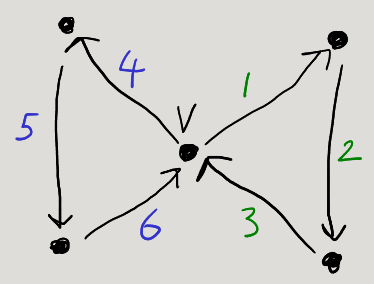
\includegraphics[scale=0.5]{even-length.png}
\end{figure}
\end{proof}

\subsection{(b)}
Give an example of a digraph in which a vertex $v$ is on an odd-length closed walk but not on an odd-length cycle.
\begin{proof}
Below the vertex $v$ is on an odd-length closed walk: $1 \to 2 \to 3 \to 4 \to 5$. There are only two cycles: $1 \to 5$ which has even length, and $2 \to 3 \to 4$ which has odd length. $v$ is on the first cycle but not on the second one.

\begin{figure}[ht!]
\centering
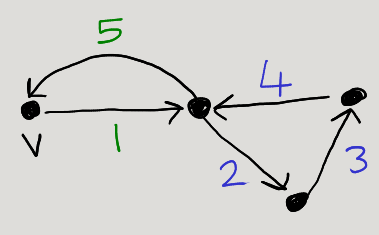
\includegraphics[scale=0.5]{odd-length-walk.png}
\end{figure}
\end{proof}

\subsection{(c)}
Prove that every odd-length closed walk contains a vertex that is on an odd-length cycle.
\begin{proof}
We argue by Strong Induction on the length of the closed walk. Define
\begin{center}
$P(n) \Coloneqq$ every closed walk of length $2n+1$ contains a vertex that is on an odd-length cycle.
\end{center}

{\bf Base Case.} $n = 0$. Every closed walk of length 1 is itself an odd-length cycle, so $P(0)$ is true.

{\bf Induction Step.} 

1. Assume $n \geq 0$ and assume $P(k)$ is true for all $k \leq n$. So every closed walk of length $2k+1$ contains a vertex that is on an odd-length cycle, for all $k \leq n$.

2. Assume $W$ is a closed walk of length $2(n+1) + 1$. Let us write:
$$
W \Coloneqq v_0 \langle v_0 \to v_1\rangle v_1 \ldots \langle v_{2n+2} \to v_{2n+3}\rangle v_{2n+3}
$$
where $v_0 = v_{2n+3}$.

3. If $W$ is itself a cycle, then $P(n+1)$ is true and we are done. So assume $W$ is not a cycle.

4. By (3) there exists a vertex $v$ on $W$ (different than the starting and ending vertex $v_0 = v_{2n+3}$) that occurs at least twice on $W$. So $W$ looks like:
$$
W \Coloneqq v_0 \langle v_0 \to v_1\rangle v_1 \ldots v \langle v \to w\rangle w \ldots x \langle x \to v\rangle v \ldots  \langle v_{2n+2} \to v_{2n+3}\rangle v_{2n+3}
$$

5. Consider the closed walk $V$ somewhere in the middle of $W$ defined by
$$
V \Coloneqq v \langle v \to w\rangle w \ldots x \langle x \to v\rangle v
$$

6. Notice that $V$ has length that is $\leq 2n+1$. If $V$ has odd-length, then by the Induction Hypothesis $V$ contains a vertex that is on an odd-length cycle, which is then also true for $W$ because $V$ is contained in $W$, and we are done.

7. So by (6) we may assume $V$ has even length of at least 2.

8. Consider the closed walk $W'$ obtained from $W$ by removing $V$:
$$
W' \Coloneqq v_0 \langle v_0 \to v_1\rangle v_1 \ldots v  \ldots  \langle v_{2n+2} \to v_{2n+3}\rangle v_{2n+3}
$$

9. By (8) and (7) $W'$ has length $\leq 2n+1$. By the Induction Hypothesis $W'$ (and therefore $W$) contains a vertex that is on an odd-length cycle.

10. So by Strong Induction, $P(n)$ is true for all $n \geq 0$. This completes the proof.
\end{proof}

\section{Problem 2}
Lemma 9.2.5 states that $dist(u, v) \leq dist(u, x) + dist(x, v)$. It also states that equality holds iff $x$ is on a shortest path from $u$ to $v$. 

\subsection{(a)}
Prove the ``iff'' statement from left to right.
\begin{proof}
1. Assume $dist(u, v) = dist(u, x) + dist(x, v)$. Want to prove $x$ is on a shortest path from $u$ to $v$.

2. $dist(u,x)$ is the length of a shortest path between $x$ and $u$. Let $P_1$ be a shortest path between $u$ and $x$. So $|P_1| = dist(u,x)$.

3. Similarly let $P_2$ be a shortest path between $x$ and $v$. So $|P_2| = dist(x,v)$.

4. Define $P \Coloneqq P_1 + P_2$ to be the path obtained by joining $P_1$ and $P_2$ at the vertex $x$.

5. Notice that by definition $|P| = |P_1| + |P_2|$, so by (2) and (3) we have $|P| = dist(u,x) + dist(x,v)$.

6. By (1) and (5) we have $|P| = dist(u,v)$.

7. By (6) $P$ is a shortest path from $u$ to $v$. And $x$ is on the path $P$, which finishes the proof.
\end{proof}

\subsection{(b)}
Prove the ``iff'' from right to left.
\begin{proof}
1. Assume $x$ is on a shortest path $P$ from $u$ to $v$. So $|P| = dist(u,v)$.

2. Write
$$
P \Coloneqq u \to v_1 \to \ldots \to v_i \to x \to v_j \to \ldots \to v_n \to v
$$

3. Split $P$ into two paths:
$$
P_1 \Coloneqq u \to v_1 \to \ldots \to v_i \to x 
$$
and
$$
P_2 \Coloneqq x \to v_j \to \ldots \to v_n \to v
$$
So the length of $P$ is the sum of the lengths of $P_1$ and $P_2$:
$$
|P| = |P_1| + |P_2|
$$

4. Notice that $P_1$ is a shortest path between $u$ and $x$ (otherwise, there is a shorter path $P_1'$ between $u$ and $x$, so $P_1' + P_2$ would be a path between $u$ and $v$ that is shorter than $P$, a contradiction).

5. Similarly, $P_2$ is a shortest path between $x$ and $v$.

6. By (4) and (5) we have $|P_1| = dist(u,x)$ and $|P_2| = dist(x,v)$.

7. By (1), (2) and (6) we have $dist(u, v) = dist(u, x) + dist(x, v)$.
\end{proof}

\section{Problem 3}
A 3-bit string is a string made up of 3 characters, each a 0 or a 1. Suppose you’d like to write out, in one string, all eight of the 3-bit strings in any convenient order. For example, if you wrote out the 3-bit strings in the usual order starting with 000 001 010 $\ldots$, you could concatenate them together to get a length $3 \cdot 8 = 24$ string that started 000001010 $\ldots$

But you can get a shorter string containing all eight 3-bit strings by starting with 00010 $\ldots$ Now 000 is present as bits 1 through 3, and 001 is present as bits 2 through 4, and 010 is present as bits 3 through 5, $\ldots$
\subsection{(a)}
Say a string is 3-good if it contains every 3-bit string as 3 consecutive bits somewhere in it. Find a 3-good string of length 10, and explain why this is the minimum length for any string that is 3-good.
\begin{proof}
0001011100 works. So does 1010001110. Now we want to show that length 10 is the minimum length. 

First, any 3-good string must contain both 000 and 111, so it must have length at least 6. 

Second, it must also contain 010, so it must have length at least 8 (by either adding 10 after 000, or adding 01 before 000, which are the only two ways of obtaining 010 with the least increase in length).

Third, it must also contain 110, so it must have length at least 9 (by adding 0 at the end of 111, which is the only way to obtain 110 with the least increase in length).

Finally, it must also contain 101 (which can only be obtained by adding one more 1 with the least increase in length), so it must have length at least 10.
\end{proof}

\begin{figure}[ht!]
\centering
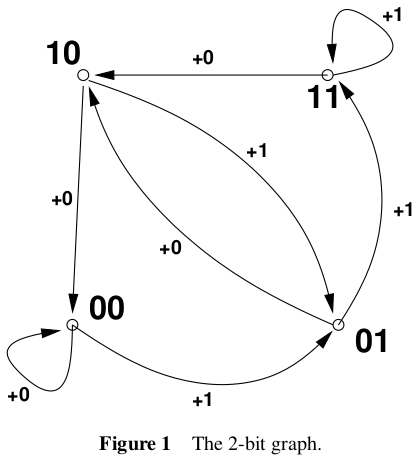
\includegraphics[scale=0.5]{2-bit-graph.png}
\end{figure}

\subsection{(b)}
Explain how any walk that includes every edge in the graph shown in Figure 1 (above) determines a string that is 3-good. Find the walk in this graph that determines your 3-good string from part (a).
\begin{proof}
There are 4 nodes, so any walk must start and finish at one of these nodes.

A walk that starts at one of these 4 nodes and includes every one of the 8 edges determines a 3-good string as follows: it starts with the 2-bit string of that node, followed by the 8 additions that come from the edges.

For example, if we start at the node 00, 

we can first follow the self-loop +0 (now our string is 000), 

then we can follow the +1 edge to the 01 node, (now our string is 0001, so it contains 001 also),

then we can follow the +0 edge to the 10 node, (now our string is 00010, so it contains 010 also),

then we can follow the +1 edge back to the 01 node, (now our string is 000101, so it contains 101 also),

then we can follow the +1 edge back to the 11 node, (now our string is 0001011, so it contains 011 also),

then we can follow the +1 self-loop at the 11 node, (now our string is 00010111, so it contains 111 also),

then we can follow the +0 edge to the 10 node, (now our string is 000101110, so it contains 110 also),

finally we can follow the +0 edge to the 00 node (now our string is 0001011100, so it contains 100 also). 

If a walk contains more than the 8 unique edges (in other words, if it includes all 8 unique edges AND ALSO repeats some of the 8 unique edges), then it will be more than sufficient for 3-goodness.
\end{proof}

\subsection{(c)}
Explain why a walk in the graph of Figure 1 (above) that includes every every edge exactly once provides a minimum-length 3-good string.
\begin{proof}
This is explained partially above in part (b). But let's explain why exactly 8 edges give us a minimum-length (10) 3-good string.

Basically, reaching any node (either by starting at that node, or arriving at that node by following an edge from another node) guarantees the 2-bit string of that node to be included.

Following the two edges +0 and +1 going out from node 10 guarantees that the string will contain 100 and 101.

Similarly, following the two edges +0 and +1 going out from node 00 guarantees that the string will contain 000 and 001.

Similarly, following the two edges +0 and +1 going out from node 01 guarantees that the string will contain 010 and 011.

Similarly, following the two edges +0 and +1 going out from node 11 guarantees that the string will contain 110 and 111.

So, following 8 edges guarantees the inclusion of all 8 3-bit strings. Including the 2-bit string at the starting node (no matter at which node we started), we get exactly 10-bit string, which has minimum-length.
\end{proof}

\subsection{(d)}
Generalize the 2-bit graph to a $k$-bit digraph, $B_k$, for $k \geq 2$, where $V(B_k) \Coloneqq \{0,1\}^k$, and any walk through $B_k$ that contains every edge exactly once determines a minimum length $(k + 1)$-good bit-string.

What is this minimum length?

Define the transitions of $B_k$. Verify that the in-degree and out-degree of every vertex is even, and that there is a positive path from any vertex to any other vertex (including itself) of length at most $k$.
\begin{proof}
The 2-bit digraph had nodes corresponding to 2-bit strings, so it had $2^{2} = 4$ nodes. 

It had $8 = 2^{2+1}$ transitions (edges).

The minimum length was equal to: the length of the 2-bit string at a starting node, plus the number of transition edges that complete the walk: $2 + 2^{2+1} = 10$.

Each node had in-degree 2, and out-degree 2. The sum of all the in-degrees was $2^{2} \cdot 2 = 8$, the sum of all the out-degrees was $2^{2} \cdot 2 = 8$, and the number of edges was also 8.

So, the $k$-bit digraph will have $2^k$ nodes, each one corresponding to one of the $2^k$ $k$-bit strings in $V(B_k) = \{0,1\}^k$. 

And it will have $2^{k+1}$ transitions (edges).

The minimum length will be: the length of the $k$-bit string at a starting node, plus the number of transition edges that complete the walk: $k + 2^{k+1}$.

Each node will have in-degree $2$, and out-degree $2$. The sum of all the in-degrees will be $2^{k} \cdot 2 = 2^{k+1}$, the sum of all the out-degrees will be $2^{k} \cdot 2 = 2^{k+1}$, and the number of edges will also be $2^{k+1}$.

Before we define the transitions of $B_k$ let's take a look at the digraph of 3-bit strings:

\begin{figure}[ht!]
\centering
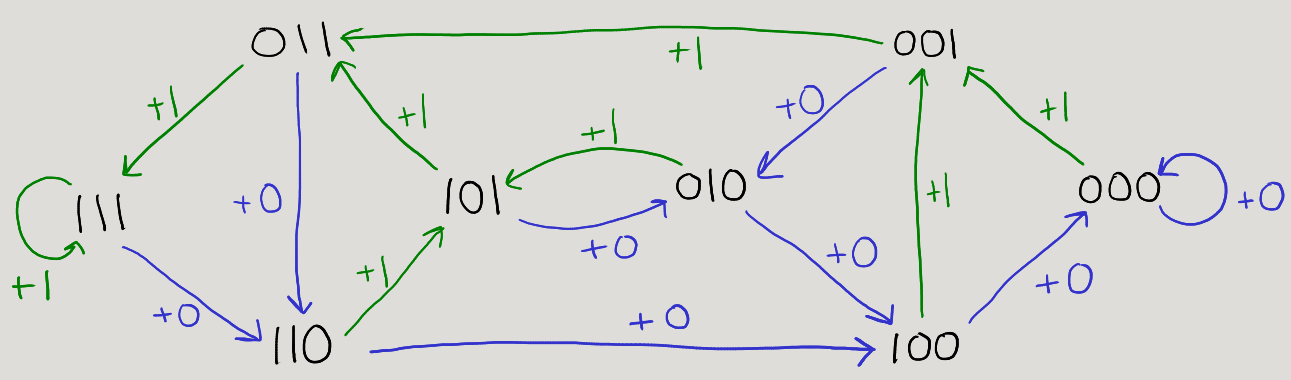
\includegraphics[scale=0.35]{3-bit-digraph.png}
\end{figure}

The transitions of $B_k$ are defined as follows. For a $k$-bit string $s \in V(B_k)$:

if $s$ ends in 0, then both of the arrows coming in to $s$ are +0;

if $s$ ends in 1, then both of the arrows coming in to $s$ are +1;

and in both cases, one of the outgoing arrows from $s$ is +0, the other +1.

Now we need to define which other $k$-bit strings are connected to $s$:

$s$ has an outgoing arrow with +0 to the $k$-bit string obtained by deleting the leftmost bit of $s$ and adding 0 to the right of $s$,

$s$ has an outgoing arrow with +1 to the $k$-bit string obtained by deleting the leftmost bit of $s$ and adding 1 to the right of $s$,

if $s$ ends with a 0, then:

$s$ has an incoming arrow with +0 from the $k$-bit string obtained by deleting the rightmost bit of $s$ and adding 0 to the right of $s$,

$s$ has an incoming arrow with +0 from the $k$-bit string obtained by deleting the rightmost bit of $s$ and adding 1 to the right of $s$,

else:

$s$ has an incoming arrow with +1 from the $k$-bit string obtained by deleting the rightmost bit of $s$ and adding 0 to the right of $s$,

$s$ has an incoming arrow with +1 from the $k$-bit string obtained by deleting the rightmost bit of $s$ and adding 1 to the right of $s$.

From these definitions it's clear that all the in-degrees and out-degrees are even.

It's also clear that there is a path from any vertex to any other vertex of length at most $k$ because: every vertex has a $k$-bit string, two different $k$-bit strings can differ in at most $k$ digits, and each edge changes 1 of the $k$ digits, so changing one vertex to the other will take at most $k$ digit swaps (in other words, going through at most $k$ edges).
\end{proof}

\section{Problem 4 (Supplemental Problem)}
In a round-robin tournament, every two distinct players play against each other just once. For a round-robin tournament with no tied games, a record of who beat whom can be described with a tournament digraph, where the vertices correspond to players and there is an edge $\langle x \to y\rangle$ iff $x$ beat $y$ in their game.

A ranking is a path that includes all the players. So in a ranking, each player won the game against the next ranked player, but may very well have lost their games against players ranked later; whoever does the ranking may have a lot of room to play favorites.

\subsection{(a)}
Give an example of a tournament digraph with more than one ranking.

\begin{proof}
Here is an example. It's a tournament with 4 players, so there are a total of 6 games played. The two different rankings are shown in separate colors; in the first, we have $b \to a \to d \to c$ so $b$ is in ``first place'' and $c$ is in ``last place''; in the second, we have $c \to b \to a \to d$ so $c$ is in ``first place'' and $d$ is in ``last place''.

\begin{figure}[ht!]
\centering
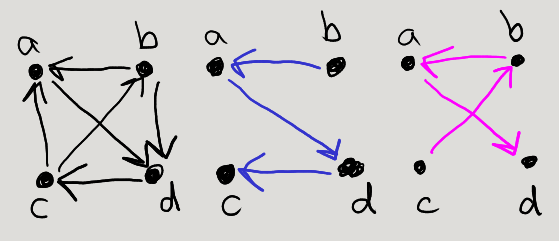
\includegraphics[scale=0.5]{digraph.png}
\end{figure}
\end{proof}

\subsection{(b)}
Prove that every finite tournament digraph has a ranking.
\begin{proof}
The proof is by induction on the number of vertices of a finite tournament digraph.

Define $P(n)$ to be the statement:
\begin{center}
$P(n) \Coloneqq $ every finite tournament digraph with $n$ vertices has a ranking.
\end{center}

{\bf Base Case} $n = 2$. Assume $G$ is a finite tournament digraph with 2 vertices $x, y$. Then $G$ has exactly one edge: either $\langle x,y \rangle$ or $\langle y,x \rangle$. In either case, that edge is a ranking: it's a path (each vertex occurs exactly once) that contains all the players ($x$ and $y$). This proves $P(2)$.

{\bf Induction Step.} 

1. Assume $n \geq 2$ and assume $P(n)$.

2. Assume $G$ is a finite tournament digraph with $n+1$ players $v_1, \ldots, v_n, v_{n+1}$.

3. Consider the finite tournament digraph $G'$ obtained from $G$ by removing $v_{n+1}$ and all the $n$ edges that are coming into, or going out from, $v_{n+1}$.

4. $G'$ has $n$ vertices. By the Induction Hypothesis $P(n)$, $G'$ has a ranking $r'$. So $r'$ is a path with $n-1$ edges that includes all of the vertices $v_1, \ldots, v_n$.

5. For the sake of convenience, write $r'$ as: 
$$
v_{i_1} \to v_{i_2} \to \ldots \to v_{i_{n-1}} \to v_{i_n}
$$ 
for some permutation $i_1, \ldots, i_n$ of $1, \ldots, n$.

6. If $v_{n+1}$ beats $v_{i_1}$ then we can add to $r'$ the edge $v_{n+1} \to v_{i_1}$ to obtain
$$
r \Coloneqq v_{n+1} \to v_{i_1} \to \ldots \to v_{i_n}
$$
which is a ranking of $G$.

Similarly, if $v_{i_n}$ beats $v_{n+1}$ then we can add to $r'$ the edge $v_{i_n} \to v_{n+1}$ to obtain
$$
r \Coloneqq v_{i_1} \to \ldots \to v_{i_n} \to v_{n+1} 
$$
which is a ranking of $G$.

7. So, by (6) we may assume that $v_{i_1} \to v_{n+1} \to v_{i_n}$.    

Now we can repeat the argument in (6) with $v_{i_2}$ and $v_{i_{n-1}}$:

If $v_{n+1}$ beats $v_{i_2}$ then we can add to $r'$ the edges $v_{i_1} \to v_{n+1}$ and $v_{n+1} \to v_{i_2}$; and remove from $r'$ the edge $v_{i_1} \to v_{i_2}$ to obtain:
$$
r \Coloneqq v_{i_1} \to v_{n+1} \to v_{i_2} \to \ldots \to v_{i_n}
$$
which is a ranking of $G$.

Similarly, if $v_{i_{n-1}}$ beats $v_{n+1}$ then we can add to $r'$ the edges $v_{i_{n-1}} \to v_{n+1}$ and $v_{n+1} \to v_{i_n}$; and remove from $r'$ the edge $v_{i_{n-1}} \to v_{i_n}$ to obtain:
$$
r \Coloneqq v_{i_1} \to v_{i_2} \to \ldots \to v_{i_{n-1}} \to v_{n+1} \to v_{i_n}
$$
which is a ranking of $G$.

8. So by (7) we may assume that $v_{i_2} \to v_{n+1} \to v_{i_{n-1}}$.

9. This process will eventually stop (somewhere ``in the middle'' of $r'$) since $r'$ is a finite path. When the process stops, there is an index $j$ such that $v_{i_j} \to v_{n+1} \to v_{i_{j+1}}$. So we can add to $r'$ the edges $v_{i_j} \to v_{n+1}$ and $v_{n+1} \to v_{i_{j+1}}$; and remove from $r'$ the edge $v_{i_j} \to v_{i_{j+1}}$ to obtain
$$
r \Coloneqq v_{i_1} \to v_{i_2} \to \ldots \to v_{i_{j}} \to v_{n+1} \to v_{i_{j+1}} \to \ldots \to v_{i_{n-1}} \to v_{i_n}
$$
which is a ranking of $G$.

10. So $G$ has a ranking, which proves $P(n+1)$. So by Induction $P(n)$ is true for all $n \geq 2$, which completes the proof.
\end{proof}

\end{document}
